\documentclass[11pt]{article}
\ifdefined\pdfinfoomitdate\pdfinfoomitdate=1\fi
\ifdefined\pdftrailerid\pdftrailerid{}\fi
\ifdefined\pdfsuppressptexinfo\pdfsuppressptexinfo=15\fi
\usepackage[T1]{fontenc}
\usepackage{lmodern}
\usepackage[margin=1.05in]{geometry}
\usepackage{amsmath,amssymb,amsthm,mathtools}
\usepackage{microtype}
\usepackage{enumitem,booktabs,array,float}
\usepackage{tikz}
\usetikzlibrary{arrows.meta,positioning}
\usepackage{xcolor}
\definecolor{linkcolor}{RGB}{20,75,105}
\usepackage[hyphens]{url}
\usepackage[colorlinks=true,linkcolor=linkcolor,citecolor=linkcolor,urlcolor=linkcolor]{hyperref}
\usepackage{bookmark}
\hypersetup{pdftitle={Symmetry of semialgebraic bounded domains with compact quotient},
  pdfauthor={OpenAI}}
\numberwithin{equation}{section}
\newtheorem{theorem}{Theorem}[section]
\newtheorem{lemma}[theorem]{Lemma}
\newtheorem{proposition}[theorem]{Proposition}
\newtheorem{corollary}[theorem]{Corollary}
\theoremstyle{definition}
\newtheorem{definition}[theorem]{Definition}
\theoremstyle{remark}
\newtheorem{remark}[theorem]{Remark}
\newcommand{\R}{\mathbb R}
\newcommand{\C}{\mathbb C}
\newcommand{\N}{\mathbb N}
\newcommand{\Z}{\mathbb Z}
\newcommand{\D}{\mathbb D}
\newcommand{\eps}{\varepsilon}
\newcommand{\abs}[1]{\lvert #1\rvert}
\newcommand{\norm}[1]{\lVert #1\rVert}
\DeclareMathOperator{\dist}{dist}
\DeclareMathOperator{\Reop}{Re}
\DeclareMathOperator{\Imop}{Im}
\DeclareMathOperator{\Aut}{Aut}
\DeclareMathOperator{\supp}{supp}
\DeclareMathOperator{\tr}{tr}
\DeclareMathOperator{\diag}{diag}
\setlist{itemsep=3pt,topsep=5pt}
\setlength{\emergencystretch}{1em}
\title{Symmetry of semialgebraic bounded domains\\with compact quotient}
\author{OpenAI}
\date{September 24, 2026}

\begin{document}
\maketitle
\begin{abstract}
Every nonempty connected semialgebraic bounded open subset of a complex
affine variety admitting a properly discontinuous cocompact group of
biholomorphisms is smooth and biholomorphic to a bounded symmetric domain.
This answers the bounded-domain question of Koll\'ar and Pardon affirmatively.
\end{abstract}

\section{Introduction}
\label{sec:introduction}

A bounded symmetric domain is a bounded domain in a complex vector space
with a holomorphic involution at every point for which that point is an
isolated fixed point. Such domains are distinguished by their large
automorphism groups. A compact quotient imposes a different kind of
uniformity: every point can be moved into a fixed compact set, but the
automorphism group need not be assumed transitive. We show that a
semialgebraic realization converts this weaker uniformity into symmetry.

We regard an affine variety as a reduced complex algebraic set, and fix a
closed algebraic embedding into some \(\C^N\). A subset is semialgebraic
if it is given by a finite Boolean combination of polynomial equalities
and inequalities in the real and imaginary coordinates. Boundedness is
in this embedding. The open set below is open in the complex-space
topology; it need not initially be a manifold.

\begin{theorem}\label{thm:main}
Let \(U\) be a nonempty connected semialgebraic bounded open subset of a
complex affine variety. Suppose that a group \(\Gamma\) of
biholomorphisms acts properly discontinuously on \(U\) and that
\(U/\Gamma\) is compact. Then \(U\) is smooth and is biholomorphic to a
bounded symmetric domain.
\end{theorem}

Proper discontinuity is understood as properness of the action when
\(\Gamma\) has the discrete topology. Finite stabilizers are allowed.
No smoothness or projectivity assumption is made on the quotient. We use
the usual nonempty-domain convention; a connected zero-dimensional
\(U\) is a point and gives the zero-dimensional case of the theorem.

\paragraph{The problem and its predecessors.}
Koll\'ar and Pardon posed the bounded semialgebraic affine-domain question
in their study of algebraic varieties with semialgebraic universal
covers~\cite[arXiv version~2, Question~25]{KP2012}. Theorem~\ref{thm:main} answers that
question affirmatively. It concerns the geometry of the domain itself:
the affine ambient variety may be singular, and the compact quotient may
have finite quotient singularities. The semialgebraic hypothesis describes
the domain in one affine embedding; it imposes no algebraicity requirement
on the biholomorphisms in $\Gamma$. This bounded-domain question is distinct
from the broader universal-cover classification proposed in the same paper.
The companion article~\cite[Theorem~1.1]{OpenAISemialgebraicCovers2026}
establishes that classification for ordinary universal covers of connected
normal projective complex varieties. The proof below is independent of
that classification.

The question arises when one tries to pass from quasi-projective universal
covers to semialgebraic ones. As Koll\'ar and Pardon explain
\cite[arXiv version~2, Section~3, p.~13]{KP2012}, when a free properly
discontinuous action on a bounded open subset of a Stein manifold has
compact quotient, that quotient is projective and its canonical bundle
is ample. Consequently, the argument that excludes varieties of general
type in the quasi-projective-cover setting does not extend to this case.
The bounded-domain question asks what geometry replaces that exclusion.

Earlier rigidity theorems explain why boundary geometry is a natural way
to approach the problem. Wong's characterization of the ball and Rosay's
subsequent localization theorem show that a bounded domain with an
automorphism orbit accumulating at a $C^2$ strongly pseudoconvex boundary
point is biholomorphic to a ball~\cite{Wong1977,Rosay1979}. Rosay's argument
uses a holomorphic peak function to force an entire sequence of
automorphisms toward the same boundary point
\cite[Section~3, Lemma~2]{Rosay1979}. The first step of our proof extends
this localization mechanism to an open subset of a possibly singular,
nonnormal affine variety. A polynomial factor first excludes the ambient
singular locus, and bounded holomorphic functions on finite branched charts
provide the compactness needed before smoothness has been established.

Frankel proved that a convex hyperbolic domain with compact quotient is
biholomorphic to a bounded symmetric domain
\cite[Theorem~1]{Frankel1989}. He also treated a broader condition on
the boundary, called $h$-convexity
\cite[Theorem~2.6 and Definition~7.3]{Frankel1989}. His proof relates
compact-quotient rigidity to limits of rescaled automorphisms
\cite[Section~3]{Frankel1989}. Although his initial theorem is stated for
a free action, he explicitly removes that restriction later in the paper
\cite[p.~144, following Lemma~11.8]{Frankel1989}. Thus finite stabilizers
are part of the earlier rigidity picture as well. The issue here is to
extract the appropriate model from semialgebraicity without assuming
convexity or a boundary regularity condition. In the setting of a bounded
domain covering a compact complex manifold, Zimmer proved that a
$C^{1,1}$ boundary already forces the domain to be a ball
\cite[Theorem~1.1]{Zimmer2021}. That regularity theorem and the present
semialgebraic theorem apply under different hypotheses.

An important earlier rigidity theorem is due to Vey: a divisible
generalized Siegel domain is symmetric~\cite[Theorem~1 and the following
paragraph]{Vey1970}. This class was introduced by Kaup, Matsushima, and
Ochiai, as Vey recalls at the start of his paper. Here divisibility means a properly discontinuous
action with a compact covering set; it does not require a free action.
The present problem is to reach a domain to which that theorem applies
without assuming a regular boundary, convexity, or homogeneity. We do so
by a rescaling construction and verify Vey's hypotheses explicitly in
Section~\ref{sec:symmetry}.

Semialgebraicity provides finite geometric descriptions, but it does not
make the relevant boundary a smooth hypersurface. Corners may have several
complex-normal directions, and their normal fibers can shrink at rates
that depend on the tangential parameters. The proof consequently uses
compatible Nash cell decomposition and semialgebraic selection
\cite[Sections~1.1--1.2]{Coste2005}, followed by a parameter argument that
keeps the tangential variables and the scale together. Analytic discs then
turn a family of approaching interior graphs into balls with a definite
size after dilation. This is the step that prevents the normal limit from
collapsing.

\paragraph{The boundary construction.}
In positive dimension, the essential intermediate result is a global
equivalence, for integers \(m\geq0\) and \(k\geq1\) with
\(m+k=\dim_\C U\),
\[
 U\simeq
 \{(z,w)\in\C^m\times\C^k:
        \Imop w-H(z,z)\in C\},
\]
where \(C\subset\R^k\) is a nonempty connected open cone and
\(H:\C^m\times\C^m\to\C^k\) is a vector of Hermitian forms.
Independent real linear functionals on
the normal variables are strictly positive on \(C\) and give
positive-definite scalar Hermitian forms after composition with \(H\).
The displayed domain is invariant under real translations of \(w\),
scalar unit rotations of \(z\), and the weighted dilations
\((z,w)\mapsto(\sqrt r\,z,rw)\), \(r>0\).
The support inequalities give a bounded realization in \(\C^{m+k}\).
Together with the transferred compact quotient, these are precisely the
properties used in Vey's theorem. They are conclusions of the construction.

Two features of that construction are useful beyond a smooth
hypersurface setting. First, semialgebraicity supplies a boundary
stratum at which normal-offset distance functions have limits jointly
in the tangential parameter and the scale. A measure argument selects
such a point together with enough independent holomorphic supports to
control every complex-normal direction. Second, analytic discs produce
interior slice balls whose radius is comparable to their distance from
that point. This rules out collapse of the normal limit even when the
boundary has higher real codimension. Both statements are formulated
with the parameter uniformity needed for weighted rescaling.

\paragraph{Proof outline.}
Section~\ref{sec:geometry} first removes the singularities of \(U\).
A polynomial-weighted maximum gives a peak at a smooth ambient point;
cocompactness moves each point of \(U\) into that smooth
neighborhood. The same compact-covering property makes the intrinsic
chain-of-discs distance proper and gives a continuity principle for
analytic-disc deformations.

Section~\ref{sec:preparation} constructs the supported boundary point
and the joint normal-offset limits. Section~\ref{sec:noncollapse} proves
that the limiting interior contains an open cone. In
Section~\ref{sec:scaling}, tangential dilation by \(t^{-1/2}\) and normal
dilation by \(t^{-1}\) yield the quadratic model. The proof uses both
interior and excluded-point convergence: normal-family limits of the maps and
their inverses give a global biholomorphism, not merely an embedding
into a candidate model. Section~\ref{sec:symmetry} then applies Vey's
theorem and completes the proof.

Figure~\ref{fig:proof} records where the two boundary inputs enter. The
independent supports control the scaled automorphisms in every normal
direction; the interior balls establish that there is a nonempty model to
which their inverses can be applied. Both sides of the set convergence are
then needed to identify the entire image of the limiting map.

\begin{figure}[H]
\centering
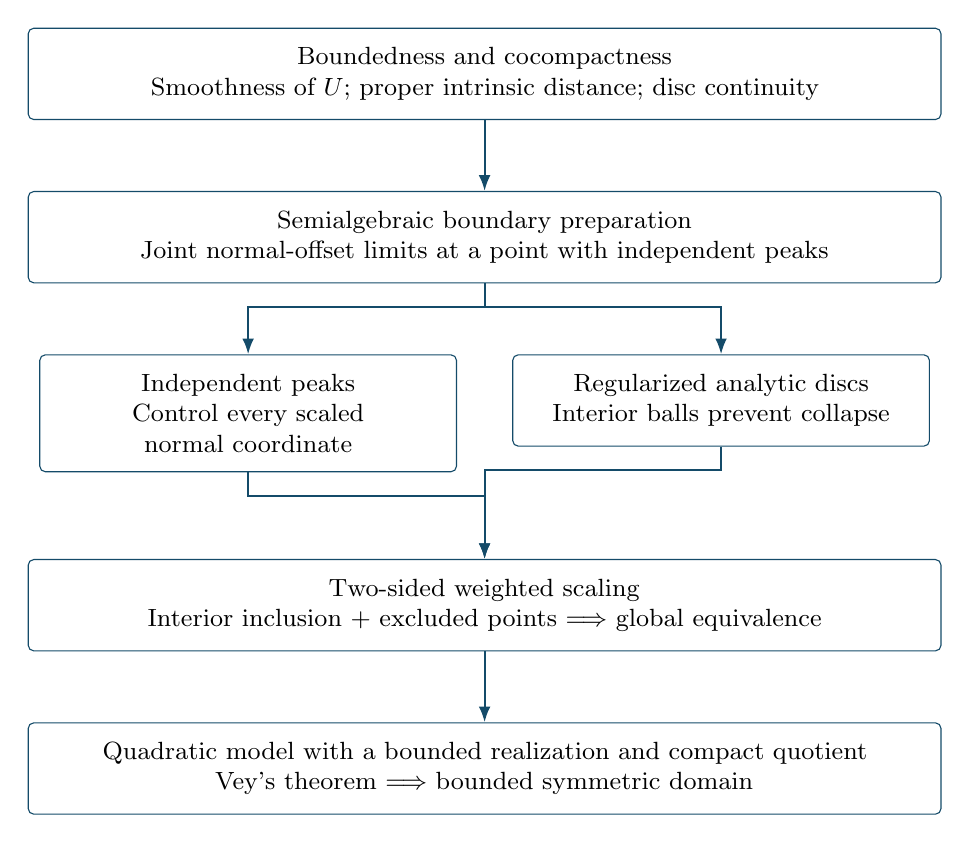
\begin{tikzpicture}[
  box/.style={draw=linkcolor,rounded corners=2pt,align=center,
    font=\small,text width=4.8cm,inner sep=7pt},
  wide/.style={box,text width=11.1cm},
  flow/.style={-{Latex[length=2mm]},draw=linkcolor,thick},
  node distance=9mm and 7mm]
  \node[wide] (smooth) {Boundedness and cocompactness\\
    Smoothness of $U$; proper intrinsic distance; disc continuity};
  \node[wide,below=of smooth] (boundary) {Semialgebraic boundary preparation\\
    Joint normal-offset limits at a point with independent peaks};
  \node[box,anchor=north east] (supports)
    at ([xshift=-3.5mm,yshift=-9mm]boundary.south)
    {Independent peaks\\Control every scaled normal coordinate};
  \node[box,anchor=north west] (discs)
    at ([xshift=3.5mm,yshift=-9mm]boundary.south)
    {Regularized analytic discs\\Interior balls prevent collapse};
  \node[wide,below=35mm of boundary] (scaling)
    {Two-sided weighted scaling\\
    Interior inclusion $+$ excluded points $\Longrightarrow$ global equivalence};
  \node[wide,below=of scaling] (vey)
    {Quadratic model with a bounded realization and compact quotient\\
    Vey's theorem $\Longrightarrow$ bounded symmetric domain};
  \draw[flow] (smooth) -- (boundary);
  \draw[flow] (boundary.south) -- ++(0,-3mm) -| (supports.north);
  \draw[flow] (boundary.south) -- ++(0,-3mm) -| (discs.north);
  \draw[flow] (supports.south) -- ++(0,-3mm) -| (scaling.north);
  \draw[flow] (discs.south) -- ++(0,-3mm) -| (scaling.north);
  \draw[flow] (scaling) -- (vey);
\end{tikzpicture}
\caption{The two boundary inputs have different roles. Peaks bound the
forward scaling maps, while discs ensure a nonempty normal interior.
The two-sided convergence then identifies the global quadratic model.
}
\label{fig:proof}
\end{figure}


\section{Smoothness and a proper intrinsic distance}\label{sec:geometry}

We first establish two consequences of boundedness and cocompactness that do
not use semialgebraicity: the open set is smooth, and analytic discs cannot
escape it during a deformation whose boundaries remain inside.  These facts
will allow us to work at the boundary without assuming its regularity.
The peak-function localization has its classical predecessor in Rosay's
argument at a strictly pseudoconvex boundary point
\cite[Section~3, Lemma~2]{Rosay1979}. Here a finite-projection argument
allows the localization to begin before the open set is known to be smooth.

Embed the initial reduced affine variety in $\C^N$ in coordinates in which
$U$ is bounded.  Its closure $\overline U$ is compact.  There is a compact set
$K\subset U$ such that $\Gamma K=U$.  Indeed, the quotient map is open, and
the images of relatively compact open neighborhoods in $U$ cover $U/\Gamma$;
finitely many suffice.  Their closures give $K$.  This argument does not
require the action to be free.

\begin{lemma}\label{lem:singular-montel}
Let $W$ be an open subset of a reduced complex affine algebraic set.  The
family of holomorphic functions $h$ on $W$ with $|h|\leq 1$ is locally
equicontinuous.  Every sequence in this family has a subsequence converging
uniformly on compact subsets to a continuous function $h_\infty$.
If $h_\infty(q)=1$ at a point $q\in W$, then $h_\infty=1$ in a neighborhood
of $q$.  In particular, if $W$ is connected, then $h_\infty\equiv 1$.
\end{lemma}

\begin{proof}
We give the argument at a possibly singular and nonnormal point $q$.  Work
first on one irreducible algebraic component $V_0$ through $q$, of positive
dimension $d$.  Noether normalization
\cite[Lemma~10.115.4, Tag~00OY]{StacksNoether} gives a finite algebraic map
$\pi:V_0\to\C^d$.  Translate so that $\pi(q)=0$.  By properness and
finiteness, we may restrict over a sufficiently small polydisc $B$ about $0$
and retain just the part $\Omega$ near $q$, with
\[
  \pi:\Omega\longrightarrow B\quad\hbox{proper and finite},
  \qquad \pi^{-1}(0)\cap\Omega=\{q\},\qquad \Omega\subset W.
\]
To make this restriction, take disjoint neighborhoods of the finitely many
points over $0$ and shrink $B$ until its entire inverse image lies in their
union.  The part near $q$ is then both open and closed in that inverse image.
Outside a proper algebraic hypersurface $E$ in $B$, the restricted map is a
covering with a fixed number $r\geq1$ of holomorphic sheets.  This follows
also directly from separability of the finite function-field extension:
discard the denominators and discriminant of a primitive element.

For $|h|\leq1$, form the monic polynomial of its sheet values,
\[
  P_h(z,T)=\prod_{x\in\pi^{-1}(z)\cap\Omega}(T-h(x))
           =T^r+\sum_{\nu=0}^{r-1}a_{\nu,h}(z)T^\nu,
  \qquad z\in B\setminus E.
\]
The coefficients are single-valued holomorphic functions bounded by
constants depending only on $r$.  They extend holomorphically across $E$
by the removable-singularity theorem for bounded holomorphic functions.
One elementary proof uses a complex line through the point that is not
contained in $E$, a small circle on that line missing $E$, and the Cauchy
integral on nearby parallel circles.  Properness and continuity of $h$ give
\[
                         P_h(0,T)=(T-h(q))^r.
\]
The polynomial identity $P_h(\pi(x),h(x))=0$ holds on all of $\Omega$ by
continuity, since the sheet locus is dense.  Cauchy estimates for the
uniformly bounded coefficients, on a smaller polydisc, therefore yield
\[
  |h(x)-h(q)|^r
   =|P_h(0,h(x))-P_h(\pi(x),h(x))|
   \leq C\|\pi(x)\|.
\]
Here $C$ is independent of $h$.  This proves equicontinuity at $q$ on $V_0$.
There are only finitely many components through $q$; applying the argument
to each proves the assertion on their union.  A zero-dimensional component
requires no argument.  Local compactness, a countable compact exhaustion,
and the Arzel\`a--Ascoli theorem now give compact convergence of a subsequence.

For the maximum assertion, use the same chart and consider the sheet
average
\[
  b_h(z)=\frac1r\sum_{x\in\pi^{-1}(z)\cap\Omega}h(x).
\]
It extends holomorphically to $B$, satisfies $|b_h|\leq1$, and has
$b_h(0)=h(q)$.  If $h_j\to h_\infty$ locally uniformly and
$h_\infty(q)=1$, ordinary normal-family compactness on $B$ gives, after
another extraction, a holomorphic limit of the sheet averages with value
$1$ at $0$.  The usual
maximum principle makes that limit identically $1$.  On every regular fiber,
an average of numbers in the closed unit disc can equal $1$ only if every
number equals $1$.  Thus $h_\infty=1$ on the sheet locus near $q$, hence
everywhere near $q$ by continuity.  Apply this on every component through
$q$.  Finally, $\{h_\infty=1\}$ is both closed and open in $W$, which proves
the connected case.  No identification of weakly holomorphic functions
with holomorphic functions on a nonnormal space was used.
\end{proof}

\begin{proposition}\label{prop:smoothness}
If $U$ is not a point, then it is a complex manifold of positive dimension
and lies in the smooth locus of a single irreducible component $V$ of the
ambient variety.
\end{proposition}

\begin{proof}
Choose a positive-dimensional irreducible component $V_0$ whose smooth
points not shared with another component meet $U$.  Such a component exists:
these points are dense in each positive-dimensional component, whereas a
zero-dimensional irreducible component is isolated and cannot meet the
connected nonsingleton $U$.  There is a polynomial $P$ vanishing on the
other components and on the singular locus of $V_0$, but not identically on
$V_0$.  In particular, $P$ is nonzero somewhere in $U$.

Maximize $\log|P(q)|+\|q\|^2$ on $\overline U$, with value $-\infty$ at
zeros of $P$.  A maximizer $p$ has $P(p)\ne0$, so it is a smooth, unshared
point of $V_0$.  It belongs to $\partial U$: near such a point the function
is strictly plurisubharmonic, and hence cannot have an interior maximum.
The entire function
\[
  h(q)=\frac{P(q)}{P(p)}
          \exp\bigl(2\overline p\cdot(q-p)\bigr)
\]
satisfies
\begin{equation}\label{eq:initial-peak}
  |h(q)|\leq \exp\bigl(-\|q-p\|^2\bigr)
  \quad(q\in\overline U),\qquad h(p)=1.
\end{equation}
Indeed, the logarithm of the left-hand side is at most
$\|p\|^2-\|q\|^2+2\operatorname{Re}(\overline p\cdot(q-p))$.

Choose $q_j\in U$ tending to $p$, and write $q_j=\gamma_j k_j$ with
$k_j\in K$.  After extraction, $k_j\to k\in K$, and
Lemma~\ref{lem:singular-montel} gives locally uniform convergence of
$h\circ\gamma_j$.  Equicontinuity at the moving points $k_j$ shows that
the limit has value $1$ at $k$.  It is therefore identically $1$ on $U$.
Equation~\eqref{eq:initial-peak} implies that $\gamma_j$ converges to $p$
uniformly on every compact subset of $U$.

For each $q\in U$, the point $\gamma_j(q)$ eventually lies in a smooth
ambient neighborhood of $p$.  Since a biholomorphism preserves smoothness
of the complex space, $q$ is smooth.  A smooth point belongs to exactly one
irreducible component of the ambient variety; the component is locally
constant on $U$, and hence constant by connectedness.  This gives $V$.
\end{proof}

The singleton is the zero-dimensional bounded symmetric domain, so henceforth
we work on this irreducible $V$ and put $n=\dim_\C U\geq1$.

We use Kobayashi's intrinsic distance, defined through holomorphic disc
chains~\cite[Section~2]{Kobayashi1967}. Its contraction property is built
into this definition; properness here will follow from cocompactness.
Let $\rho$ denote the Poincar\'e distance on the unit disc $\D$.  For $x,y\in U$,
define $d_U(x,y)$ as the infimum of
\[
                    \sum_{j=1}^s\rho(\alpha_j,\beta_j)
\]
over finite chains of holomorphic maps $a_j:\D\to U$ with
$a_1(\alpha_1)=x$, $a_s(\beta_s)=y$, and
$a_j(\beta_j)=a_{j+1}(\alpha_{j+1})$.  By its definition, holomorphic maps
decrease this chain-of-discs distance, and biholomorphisms preserve it.

\begin{proposition}\label{prop:proper-distance}
The function $d_U$ is a finite distance inducing the usual topology of $U$.
Every closed $d_U$-ball is compact.
\end{proposition}

\begin{proof}
Coordinate balls give finite disc chains locally, hence globally by
connectedness.  Bounded ambient coordinate functions and the Schwarz lemma
give a constant $c>0$ such that
\begin{equation}\label{eq:distance-lower-bound}
                         d_U(x,y)\geq c\|x-y\|.
\end{equation}
For example, send each bounded coordinate to $\D$; the Poincar\'e distance
there dominates a constant times Euclidean distance, and sum along a chain.
Conversely, small affine complex discs in a manifold chart give a local
upper bound tending to zero with the coordinate separation.  Thus $d_U$ is
a distance and induces the original topology.

Choose a relatively compact neighborhood of $K$ in $U$.
Equation~\eqref{eq:distance-lower-bound} and compactness of $K$ give an
$r>0$ for which every closed $r$-ball centered in $K$ lies in that
neighborhood's compact closure.  Such a ball is closed in the original
topology, hence compact.  Translating by $\Gamma$ shows that every closed
$r$-ball in $U$ is compact, with the same $r$.

We spell out why this uniform local statement implies properness.  Fix $x$,
and suppose $\overline B_{d_U}(x,R)$ is compact.  Cover it by finitely many
open $r/4$-balls centered at $x_1,\ldots,x_l$.  For
$d_U(x,y)\leq R+r/4$, choose a disc chain of total Poincar\'e length less than
$d_U(x,y)+r/4$.  Replace each disc link by a Poincar\'e geodesic segment.
If the total length exceeds $R$, the point at accumulated length $R$
lies in $\overline B_{d_U}(x,R)$, and the remaining length is less than
$r/2$.  Hence $y$ belongs to an $r$-ball centered at some $x_i$.
If the total length is at most $R$, the same conclusion is immediate.
Consequently
\[
  \overline B_{d_U}(x,R+r/4)
       \subset\bigcup_{i=1}^l\overline B_{d_U}(x_i,r).
\]
The set on the left is closed and the union on the right is compact.
Starting at $R=r$ and iterating proves compactness for every radius.
\end{proof}

\begin{lemma}[Continuity principle]\label{lem:continuity}
Let $\Omega$ be a smooth ambient coordinate neighborhood, and let
$A:[0,1]\times\overline\D\to\Omega$ be continuous, with each
$A_t=A(t,\cdot)$ holomorphic on $\D$.  Suppose
\[
  A_t(\partial\D)\subset U\quad(0\leq t\leq1),
  \qquad A_0(\overline\D)\subset U.
\]
Then $A_t(\overline\D)\subset U$ for every $t$.  In particular, this applies
to continuous deformations of closed $C^1$ analytic discs; holomorphic
extension through the boundary circle is not required.
\end{lemma}

\begin{proof}
The set $T=\{t:A_t(\overline\D)\subset U\}$ is relatively open in $[0,1]$
by compactness of the closed disc.  To see that it is closed, let
$t_j\in T$ tend to $t_*$.  The boundary condition and continuity give a
fixed collar $1-\eps\leq|\zeta|\leq1$ whose images, for $t$ near $t_*$,
lie in a compact set $L\subset U$.  Fix $\zeta_0$ in the interior of this
collar and $x_0\in U$.  By Proposition~\ref{prop:proper-distance},
$M=\max_{x\in L}d_U(x_0,x)$ is finite.  For each fixed $\zeta\in\D$,
the earlier discs take values in $U$, so Schwarz contraction gives
\[
  d_U(x_0,A_{t_j}(\zeta))
            \leq M+\rho(\zeta_0,\zeta).
\]
Properness places these values in a fixed compact subset of $U$.
Their ambient limit $A_{t_*}(\zeta)$ therefore belongs to $U$.
The boundary already lies in $U$, so $t_*\in T$.  Since $T$ is nonempty,
open, and closed in $[0,1]$, it is all of $[0,1]$.
\end{proof}

\section{Boundary preparation and independent supports}
\label{sec:preparation}

We now work in the setting furnished by Proposition~\ref{prop:smoothness}:
$V\subset\C^N$ is irreducible of complex dimension $n\geq1$, and
$U\subset V_{\mathrm{reg}}$ is a domain.  The purpose of this section is
to choose a boundary point with two simultaneous properties.  Its normal
fibers have limits uniform in the tangential parameters, and it admits
enough global holomorphic supports to control all complex-normal directions.
Neither property is asserted for an arbitrary supported boundary point.

We use the elementary semialgebraic facts of cell decomposition, selection,
and generic real analyticity.  More precisely, a semialgebraic set admits
a finite decomposition into connected real-analytic cells with algebraic
analytic parametrizations; a choice in nonempty semialgebraic fibers can
be made semialgebraically; and a semialgebraic function on an open set is
algebraic analytic off a lower-dimensional set.  For projection and
real-analytic cell decomposition, see
\cite[Sections~1.1--1.2]{Coste2005}.  These facts apply equally
to descriptions using real quantifiers.  Lower-dimensional exceptional
sets have Lebesgue measure zero.

We first separate boundary cells that admit normal graph coordinates
from those contained in a proper complex algebraic subset.  The latter
can be excluded from a maximizing construction by a polynomial factor.

\begin{lemma}[Complex rank of a boundary cell]
\label{lem:rank-dichotomy}
Let $S$ be a connected real-analytic semialgebraic cell in
$V_{\mathrm{reg}}$.  Either
\begin{equation}
 T_pS+iT_pS=T_pV
 \label{eq:generic-cell}
\end{equation}
outside an intrinsic null set of $S$, or $S$ is contained in a proper
complex algebraic subset of $V$.
\end{lemma}

\begin{proof}
Put $d=\dim_{\R}S$, and write the ambient complex coordinate functions
of an algebraic analytic parametrization of $S$ as
$q_1(s),\ldots,q_N(s)$, where $s=(s_1,\ldots,s_d)$.  Complexify the
parameters.  These germs belong to a common finite algebraic extension
of $\C(s_1,\ldots,s_d)$.  In characteristic zero, the dimension of the
span of their differentials is
\[
 \operatorname{trdeg}_{\C}\C(q_1,\ldots,q_N).
\]
Indeed, a transcendence basis among the $q_j$ has independent
differentials, as seen by extending it to a transcendence basis of the
ambient field; all remaining $q_j$ are separably algebraic over it and
add no independent differentials.  This number is also the generic
complex rank of the complexified parametrization and the dimension of
its complex Zariski closure.  The latter lies in $V$.

If the rank is less than $n$, a polynomial vanishing on that closure
but not identically on $V$ vanishes on an open patch of $S$, hence on
all of $S$ by real-analytic continuation.  If the rank is $n$, its
failure locus is defined locally by nontrivial analytic minors and has
intrinsic measure zero.  The complex image of the differential is
exactly $T_pS+iT_pS$, which proves the alternative.
\end{proof}

Decompose $\partial U\cap V_{\mathrm{reg}}$ into finitely many such
cells.  Every cell has positive real codimension, since the boundary of
an open set has empty interior.  On a cell satisfying
Equation~\eqref{eq:generic-cell}, write
\[
 k=2n-\dim_{\R}S,\qquad m=n-k,
 \qquad 1\leq k\leq n.
\]
At a point satisfying Equation~\eqref{eq:generic-cell}, choose
semialgebraic holomorphic coordinates, obtained locally from a linear
projection of $V$ followed by a complex-linear change, in which a patch
of $S$ is
\begin{equation}
 \operatorname{Im}w_0=\phi(s),\qquad
 s=(z_0,\operatorname{Re}w_0)\in B,
 \qquad (z_0,w_0)\in\C^m\times\C^k.
 \label{eq:boundary-graph}
\end{equation}
Here $B$ is an open real parameter box and $\phi$ is real analytic and
semialgebraic.  This follows from the real implicit function theorem
after putting the tangent space in the form
$\{\operatorname{Im}w_0=0\}$.  Shrinking the patch ensures that its
intersection with each fixed-$z_0$ slice is totally real in $\C^k$.

Choose $\rho>0$ so that the points with $s\in B$ and
$|v|<\rho$ below stay in the coordinate patch, and put
\begin{equation}
 \begin{split}
 v&=\operatorname{Im}w_0-\phi(s),\qquad
 s=(z_0,x_0),\quad x_0=\operatorname{Re}w_0,\\
 A_s&=\{v\in\R^k:|v|<\rho,\
       (z_0,x_0+i(\phi(s)+v))\in U\}.
 \end{split}
 \label{eq:offset-fibers}
\end{equation}
Thus the $A_s$ are open semialgebraic fibers, and $0\notin A_s$.
The cutoff $\rho$ will disappear under every bounded-coordinate scaling
as $t\downarrow0$.

We need two properties of these fibers at the same parameter: analytic
families of offsets in $A_s$ approaching zero, and distance functions
for the complements of $t^{-1}A_s$ that stabilize as $s$ moves and
$t$ tends to zero.  The joint limit matters because later coordinate
changes move the tangential parameter at the same time as the normal
scale.  The following parameter version of ramification supplies both
properties outside a null set.

\begin{lemma}[Ramification with parameters]
\label{lem:ramified-parameters}
Let $B\subset\R^d$ be a semialgebraic open set and let
$b:B\times(0,t_0)\to\R$ be a bounded semialgebraic function.  There is a
null set $E\subset B$ such that, for every $s_*\in B\setminus E$, there
are a neighborhood $B_*$ of $s_*$, an integer $l\geq1$, a number
$\eps>0$, and a real-analytic function $\widetilde b$ on
$B_*\times(-\eps,\eps)$ satisfying
\[
 b(s,u^l)=\widetilde b(s,u)
 \qquad(s\in B_*,\ 0<u<\eps).
\]
In particular, $b(s,t)$ has a limit as $(s,t)\to(s_*,0)$ with $t>0$,
without any restriction on the relative rates of approach.

Finitely many such functions can use a common ramification and
neighborhood.  For countably many functions there is a common full-measure
set of good points, with the conclusion applied separately to each
function; no common ramification or neighborhood is asserted.
\end{lemma}

\begin{proof}
Use cylindrical decomposition with $s$ preceding $t$.  Away from a
lower-dimensional subset of $B$, the region immediately above $t=0$
lies in a cell on which $b$ is an algebraic analytic branch.  Locally at
such an $s_*$, shrink to a rectangle $B_*\times(0,\eps_0)$ on which
this holds.  Choose a square-free polynomial equation
\[
 R(s,t,b(s,t))=0
\]
with polynomial coefficients in $(s,t)$ and nonzero leading coefficient
and discriminant in the last variable.  Remove the zero sets of the
first nonzero $t$-coefficients of these latter two polynomials.  After
shrinking again, each is a power of $t$ times a nonvanishing holomorphic
function on a complex $s$-polydisc times a complex $t$-disc.

For $t\ne0$ the roots therefore form a finite unramified covering of
this product with the $t$-origin deleted.  The $s$-polydisc is simply
connected, so its monodromy is generated by one finite permutation around
$t=0$.  The substitution $t=u^l$ kills this permutation for some $l$.
The chosen branch becomes holomorphic for $u\ne0$.  The polynomial root
bound, applied after division by the leading coefficient, bounds this
branch by $C|u|^{-M}$ on a smaller complex polydisc, for some finite $M$.
Thus it has at worst a pole at $u=0$, whose negative Laurent coefficients
are holomorphic in $s$.  Boundedness of the original function for real
$s$ and positive $u$ makes those coefficients vanish for every real $s$
in the rectangle.  They vanish identically by holomorphic uniqueness.
The branch consequently extends holomorphically through $u=0$, giving
the stated real-analytic extension.

There are only finitely many decomposition branches and exceptional
polynomial zero sets.  This proves the assertion outside a null set.
For finitely many functions take a common multiple of their exponents
and shrink the neighborhoods.  For countably many, discard the union
of their exceptional null sets; the individual conclusions suffice.
\end{proof}

\begin{proposition}[Generic boundary data]
\label{prop:boundary-data}
In the coordinates of Equation~\eqref{eq:boundary-graph}, almost every
$s_*\in B$ has the following two properties.
\begin{enumerate}[label=\textup{(\roman*)}]
\item There are a neighborhood $B_*\subset B$ of $s_*$, a number
$\eps>0$, and a real-analytic map
$\psi:B_*\times(-\eps,\eps)\to\R^k$ such that
\[
 \psi(s,0)=0,\qquad
 \psi(s,u)\in A_s\quad(s\in B_*,\ 0<u<\eps).
\]
\item Set
\[
 E(s,t)=\R^k\setminus t^{-1}A_s,
 \qquad d(s,t;v)=\min\{1,\operatorname{dist}(v,E(s,t))\}.
\]
There is a $1$-Lipschitz function $d_*:\R^k\to[0,1]$ such that,
for every compact $L\subset\R^k$,
\begin{equation}
 \lim_{\substack{s\to s_*\\t\downarrow0}}
       \sup_{v\in L}|d(s,t;v)-d_*(v)|=0.
 \label{eq:joint-offset-limit}
\end{equation}
The set $F=\{v:d_*(v)=0\}$ is a closed cone, invariant under every
positive real dilation, and $0\in F$.
\end{enumerate}
In particular, for every sequence $s_j\to s_*$, $t_j\downarrow0$,
and $v_j\to v$, one has $d(s_j,t_j;v_j)\to d_*(v)$.  If $v\in F$,
then
\[
 \operatorname{dist}(v_j,E(s_j,t_j))\longrightarrow0.
\]
If $v\notin F$, some fixed ball about $v$ is contained in
$t_j^{-1}A_{s_j}$ for all sufficiently large $j$.
\end{proposition}

\begin{proof}
The function
\[
 a(s)=\min\{1,\operatorname{dist}(0,A_s)\},
\]
with value $1$ for an empty fiber, is semialgebraic and continuous on
an open full-measure subset $B'\subset B$.  It is zero there.  In fact,
if $a(s_0)>0$ at a continuity point, it is bounded below near $s_0$;
but the boundary point with parameters $(s_0,0)$ is a limit of points
of $U$, whose parameters $(s_j,v_j)$ satisfy $s_j\to s_0$ and
$v_j\to0$.  This is a contradiction.

On $B'\times(0,t_0)$ semialgebraic selection therefore supplies
$v(s,t)\in A_s$ with $|v(s,t)|<t$.  Apply
Lemma~\ref{lem:ramified-parameters} to its finitely many coordinates.
At almost every $s_*$ this gives a jointly analytic
$\psi(s,u)=v(s,u^l)$.  The bound $|\psi(s,u)|<u^l$ proves
$\psi(s,0)=0$ for every $s$ in its neighborhood.  This proves (i).

For (ii), apply Lemma~\ref{lem:ramified-parameters} separately to
$d(s,t;v)$ for every $v\in\mathbb{Q}^k$.  Their exceptional sets have
a null union.  At a remaining $s_*$, each rational test has a limit
along every joint approach $(s,t)\to(s_*,0)$, $t>0$.  For every $s,t$,
\[
 |d(s,t;v)-d(s,t;v')|\leq |v-v'|.
\]
The rational limits therefore extend uniquely to a $1$-Lipschitz
function $d_*$ on $\R^k$.  A finite rational net in a compact set,
together with this inequality, proves
Equation~\eqref{eq:joint-offset-limit}.  Notice that this argument
uses only finitely many test neighborhoods at a time; it does not
require a common neighborhood for all rational tests.

The zero set $F$ is closed and contains $0$, since $0\in E(s,t)$.
For $c>0$ the exact identity
\[
 E(s,ct)=c^{-1}E(s,t)
\]
shows, on taking $s=s_*$ and $t\downarrow0$, that the distance from
$v$ to the left-hand side tends to zero if and only if the distance
from $cv$ to $E(s_*,t)$ does.  Truncation at $1$ does not affect
vanishing of a limit.  Consequently $v\in F$ if and only if $cv\in F$.

The assertion for moving vectors follows from the same Lipschitz
inequality.  If $d_*(v)=0$, convergence of the truncated distance to
zero is convergence of the untruncated distance to zero.  If
$d_*(v)>0$, the distance of $v$ from $E(s_j,t_j)$ is eventually at
least $d_*(v)/2$, so any smaller fixed ball is in the scaled interior.
\end{proof}

Using countably many patches of the form
Equation~\eqref{eq:boundary-graph}, we obtain an intrinsic full-measure
set of points on every cell in the first alternative of
Lemma~\ref{lem:rank-dichotomy}, each with the data of
Proposition~\ref{prop:boundary-data}.  Call these points \emph{good}.
The cone $F$ at a good point might still equal all of $\R^k$;
Proposition~\ref{prop:noncollapse} will rule this out.  We first choose
a good point carrying independent supports.

\begin{proposition}[A good supported point]
\label{prop:supported-point}
There are a boundary cell $S$ in the first alternative of
Lemma~\ref{lem:rank-dichotomy}, a good point $p\in S$, and
$k=2n-\dim_{\R}S$ entire functions $h_1,\ldots,h_k$ on $\C^N$
such that
\begin{equation}
 h_j(p)=1,\qquad
 |h_j(q)|\leq\exp(-|q-p|^2)\quad(q\in\overline U),
 \qquad 1\leq j\leq k.
 \label{eq:peak}
\end{equation}
The real covectors
\[
 \left.d\log|h_j|\right|_{T_pV}
\]
are linearly independent and annihilate $T_pS$.  Consequently, in
coordinates $(z,w)\in\C^{n-k}\times\C^k$ centered at $p$ with
$T_pS=\{\operatorname{Im}w=0\}$, their holomorphic logarithmic
differentials have the form
\[
 d\log h_j(p)=i\beta_j\,dw,
\]
where the $\beta_j$ are linearly independent real rows.
\end{proposition}

\begin{proof}
We vary the real linear term in the weighted maximum used in the
smoothness proof.  We seek one good point at which the maximum is
attained for a positive-measure set of linear terms, measured within
the set of all terms making that point critical on its boundary cell.
The corresponding conormals will provide $k$ independent supports.

Choose a polynomial $P$ vanishing on $V_{\mathrm{sing}}$ and on the
proper complex algebraic subsets containing all cells in the second
alternative of Lemma~\ref{lem:rank-dichotomy}, but not identically on
$V$.  Such a polynomial exists because the union is finite and $V$ is
irreducible.  For $a\in\C^N$, maximize on the compact set
$\overline U$ the upper-semicontinuous function
\[
 \Phi_a(q)=\log|P(q)|+|q|^2+\operatorname{Re}(a\cdot q),
\]
with value $-\infty$ where $P=0$.  Its maximum $M(a)$ is finite,
because $P$ is not identically zero on the open set $U$.  Every
maximizer has $P\ne0$, lies in $V_{\mathrm{reg}}$, and belongs to
$\partial U$: on the smooth locus with $P\ne0$, strict
plurisubharmonicity forbids an interior maximum.  Thus every maximizer
lies on a retained boundary cell.

Fix one retained cell $S$, of real dimension $d$, and restrict to
$S^\circ=S\cap\{P\ne0\}$.  Its critical-pair space is
\[
 \mathcal E_S=
 \{(p,a)\in S^\circ\times\C^N:
                  d(\Phi_a|_S)_p=0\}.
\]
Ambient real linear functionals restrict onto $T_p^*S$, so these are
$d$ independent real affine equations on the $2N$ real coordinates
of $a$.  Therefore $\mathcal E_S\to S^\circ$ is a smooth affine
bundle with fiber dimension $2N-d$ and total dimension $2N$.

The subset $\mathcal M_S\subset\mathcal E_S$ of actual maximizers
is Borel.  Indeed, $M(a)$ is Lipschitz in $a$, since
\[
 |M(a)-M(a')|
 \leq\bigl(\sup_{q\in\overline U}|q|\bigr)|a-a'|,
\]
and $\mathcal M_S$ is defined by the continuous equality
$\Phi_a(p)=M(a)$ on $\mathcal E_S$.  Projection
$\mathcal E_S\to\C^N$ is a smooth map between manifolds of the
same real dimension and sends null sets to null sets: in countably
many relatively compact coordinate charts it is Lipschitz.  Its
restrictions to the finitely many sets $\mathcal M_S$ cover all of
$\C^N$.  Hence at least one $\mathcal M_S$ has positive measure in
$\mathcal E_S$.

In local bundle coordinates, the points lying over the nongood null
subset of $S$ form a null set, by Fubini.  Applying Fubini again to
$\mathcal M_S$, in countably many bounded bundle charts, gives a
good point $p$ for which the set of actual maximizing parameters in
the critical fiber has positive $(2N-d)$-dimensional measure.  Fix
this $p$ and write that subset as $\mathcal A_p$.

Each $a\in\mathcal A_p$ supplies the entire function
\[
 h_a(q)=\frac{P(q)}{P(p)}
       \exp\bigl((2\overline p+a)\cdot(q-p)\bigr).
\]
The inequality $\Phi_a(q)\leq\Phi_a(p)$ gives
\[
 \log|h_a(q)|
 \leq |p|^2-|q|^2
       +2\operatorname{Re}\bigl(\overline p\cdot(q-p)\bigr)
 =-|q-p|^2,
\]
with the desired modulus inequality also at $P(q)=0$.

The affine map from the full critical fiber to the conormal space
\[
 a\longmapsto
 \left.d\log|h_a|\right|_{T_pV}
 \in N_p^*S
 :=\{\lambda\in T_p^*V:\lambda|_{T_pS}=0\}
\]
is surjective.  Indeed, on $T_pV$,
\[
 d\log|h_a|_p
   =d(\log|P|+|q|^2)_p+\operatorname{Re}(a\cdot dq).
\]
For any $\lambda\in N_p^*S$, extend
$\lambda-d(\log|P|+|q|^2)_p$ to an ambient real linear functional
$\operatorname{Re}(a\cdot dq)$.  The resulting total differential is
$\lambda$, so its restriction to $T_pS$ vanishes and $a$ belongs to
the critical fiber.  Since
$\dim_{\R}N_p^*S=k$, the inverse image of any proper linear
subspace of $N_p^*S$ has measure zero in the critical fiber.
The positive-measure set $\mathcal A_p$ cannot be contained in such
an inverse image.  Selecting successively outside the span already
chosen gives $k$ independent conormals and corresponding functions
$h_1,\ldots,h_k$.

Finally choose the local branches of $\log h_j$ with value zero
at $p$.  Their real differentials vanish on
$\C^{n-k}\times\R^k=T_pS$.  Complex linearity forces the
$dz$ coefficients to be zero and the $dw$ coefficients to be
purely imaginary.  Independence of the real conormals is exactly
independence of the resulting real rows $\beta_j$.
\end{proof}

Fix the resulting $p$, its chart $(z_0,w_0)$, the data
$s_*,\psi,F$ of Proposition~\ref{prop:boundary-data}, and the
support functions for the rest of the proof.

\section{An open cone of limiting interior}\label{sec:noncollapse}

The excluded cone supplied by Proposition~\ref{prop:boundary-data} could,
at this stage, be all of $\R^k$.  We rule this out by constructing actual
interior balls whose radii are comparable to their distance from the chosen
boundary point.  The analytic interior graphs and the continuity principle
are the essential inputs; the supporting functions will enter only in the
next section.
The construction uses the analytic-disc method introduced by
Bishop~\cite{Bishop1965}. In particular, the nonlinear boundary equation
expresses the real part in terms of the imaginary part through harmonic
conjugation; see Hill--Taiani~\cite[Section~2, Equation~(2.1) and
Proposition~2.1, pp.~330--331]{HillTaiani1978} for its
classical formulation. We prove here the parameter estimates and the
regularization needed to obtain included balls from the approaching graphs.

We first isolate the analytic-disc construction.  All balls in this section
are Euclidean balls, with the real or complex ambient space indicated by
their centers.  In the application, we fix a complex-normal slice through
the chosen boundary point and straighten its totally real boundary graph.
The approaching interior graphs then satisfy the hypotheses of the lemma
below.  A ball in this slice will give a ball in a normal-offset fiber,
which the joint limits of Section~\ref{sec:preparation} can detect.

\begin{lemma}[Interior balls from approaching graphs]\label{lem:disc-family}
Let $\Omega$ be open in a neighborhood of $0\in\C^k$.  Assume that the
continuity principle of Lemma~\ref{lem:continuity} holds for continuous
deformations of closed analytic discs contained in that neighborhood.
Suppose that $f(X,u)$ is an $\R^k$-valued real-analytic function for real
$X$ near $0$ and real $u$ near $0$, that $f(X,0)=0$, and that
\[
 X+i f(X,u)\in\Omega
 \qquad\text{for all such $X$ and all sufficiently small $u>0$.}
\]
Then there are constants $c,C,t_0>0$ and points $a_t\in\C^k$, for
$0<t<t_0$, such that
\begin{equation}\label{eq:disc-balls}
 |a_t|\le Ct,
 \qquad B(a_t,ct)\subset\Omega.
\end{equation}
The discs used to obtain these balls stay in an arbitrarily small fixed
neighborhood of $0$ after the graph neighborhood is restricted.
\end{lemma}

\begin{proof}
Write $f_u(X)=f(X,u)$.  Choose nonnegative smooth functions $\lambda_0$
and $\eta$ on the unit circle, both zero on a fixed arc about $1$, with
$\eta\not\equiv0$ and
\[
 \operatorname{supp}\eta\Subset\{\lambda_0>0\}.
\]
Set $\lambda=\alpha\lambda_0$, where the positive constant $\alpha$ will
be fixed sufficiently small.  For parameters $b,e\in\R^k$ and
$\delta\ge0$, we seek a holomorphic disc $A_{b,e,\delta}$ whose boundary
values $X+iY$ satisfy
\begin{equation}\label{eq:disc-boundary}
 X(0)=b,
 \qquad
 Y(\theta)=f_{\lambda(\theta)+\delta}(X(\theta))+
             \eta(\theta)e.
\end{equation}
Here $X(0)$ means the value at the boundary angle $\theta=0$, not the
value at the center of the disc.

The parameters $b$ and $e$ have different geometric roles.  When $\delta=0$,
the boundary arc about $1$ maps into $\R^k$, with endpoint
$A_{b,e,0}(1)=b$.  Varying $b$ moves that endpoint in the real directions;
the perturbation $\eta e$, supported away from $1$, will change the inward
radial derivative in all imaginary directions.  For $B\in\R^k$,
evaluation at $1-t$ with $b=tB$ will therefore give independent
displacements of order $t$ in all
$2k$ real directions.  We first prove this derivative assertion and then
use a positive $\delta$ to put the evaluated discs inside $\Omega$.

\paragraph{Solving the boundary equation.}
Let $\mathcal H=H^2(S^1,\R^k)$ be the real Sobolev space of functions
with two square-integrable derivatives.  The Fourier-series estimate
\[
 \sum_{j\in\Z}\frac{j^2}{(1+j^2)^2}<\infty
\]
gives the continuous embedding $\mathcal H\hookrightarrow C^1(S^1)$.
This space is a Banach algebra under multiplication.  Let $T$ be the
bounded conjugation operator which recovers the real part of a
holomorphic boundary value from its imaginary part, with real part of
mean zero, and put
\[
 \mathcal T Y=TY-(TY)(0).
\]
Thus $\mathcal T$ is bounded on $\mathcal H$, and
Equation~\eqref{eq:disc-boundary} is equivalent to
\begin{equation}\label{eq:disc-contraction}
 X=b+\mathcal T\bigl(f_{\lambda+\delta}(X)+\eta e\bigr).
\end{equation}

Here is the smallness needed for contraction.  The identity $f(X,0)=0$
gives a real-analytic factorization $f(X,u)=u\widetilde f(X,u)$.  On a fixed small
$\mathcal H$-ball of functions $X$, the product rule through two
derivatives, the embedding into $C^1$, and bounded derivatives of $\widetilde f$
give
\begin{equation}\label{eq:disc-composition-bound}
 \|f_{\lambda+\delta}(X)\|_{\mathcal H}
 +\|D_X[f_{\lambda+\delta}(X)]\|_{\mathcal L(\mathcal H)}
 \le C_0(\alpha+|\delta|).
\end{equation}
For example, both expressions contain the factor $\lambda+\delta$;
derivatives falling on that factor are also $O(\alpha+|\delta|)$.
The remaining composition and multiplication operators are uniformly
bounded on the chosen ball.  For all sufficiently small $\alpha$ and
$|\delta|$, the Lipschitz constant in
Equation~\eqref{eq:disc-contraction} is less than $1/2$.  On common
sufficiently small $b,e$ neighborhoods, its right side maps the chosen
ball into itself.  The
contraction theorem gives a unique solution $X$.

Smooth composition on $H^2$, or its direct proof by the same product
estimates, shows that this equation is smooth in $X,b,e,\delta$.
Its $X$-linearization is the identity minus an operator of norm less
than $1/2$.  The implicit function theorem therefore gives smooth
parameter dependence in $\mathcal H$.  In particular $\partial_e X$
is uniformly bounded as $\alpha$ decreases; it need not be small.
The boundary function $X+iY$ extends holomorphically to the disc and
continuously to its closure.  All these conclusions hold also with
$\lambda$ replaced by $\rho\lambda$, $0\le\rho\le1$.  Shrinking the
fixed $\mathcal H$-ball keeps every disc in the prescribed coordinate
neighborhood, by the boundary bound and the maximum principle.

\paragraph{The limiting radial derivative.}
For $\delta=0$, the function $Y$ vanishes on the fixed arc about
$\theta=0$.  Hence $A_{b,e,0}(1)=b$, and reflection across that arc
shows that the radial derivative there is purely imaginary.  More
explicitly, with $Y=Y_{b,e,0}$, the Schwarz integral gives, near $\zeta=1$,
\[
 A_{b,e,0}(\zeta)-b
 =\frac{i}{2\pi}\int_{-\pi}^{\pi}
 \left(\frac{e^{i\theta}+\zeta}{e^{i\theta}-\zeta}
       -\frac{e^{i\theta}+1}{e^{i\theta}-1}\right)
 Y(\theta)\,d\theta.
\]
There is no singularity on the support of $Y$.  Expanding the kernel
at $\zeta=1$ gives
\begin{align}
 A_{b,e,0}(1-t)
   &=b+i t D(b,e)+O(t^2),\label{eq:disc-radial}\\
 D(b,e)
   &=\frac{1}{2\pi}\int_{-\pi}^{\pi}
        \frac{2Y_{b,e,0}(\theta)}{|1-e^{i\theta}|^2}\,d\theta.
        \label{eq:disc-normal-derivative}
\end{align}
The remainder is uniform with its first derivatives in $b,e$ on a
fixed smaller parameter neighborhood.  This follows from the same
integral formula and the smooth $\mathcal H$-dependence proved above.

Differentiating Equation~\eqref{eq:disc-normal-derivative} in $e$ gives
\[
 \partial_e D(b,e)=c_\eta I+R_\alpha(b,e),
 \qquad
 c_\eta=\frac{1}{2\pi}\int_{-\pi}^{\pi}
       \frac{2\eta(\theta)}{|1-e^{i\theta}|^2}\,d\theta>0.
\]
The remainder contains $\partial_X f_{\lambda(\theta)}(X)\partial_e X$.
The first factor is $O(\alpha)$ and the second is uniformly bounded.
Their product vanishes on the arc where $\lambda=0$, so the integral
has a uniformly bounded kernel on its support.  Thus
$\|R_\alpha\|\le C_1\alpha$.  The positive constant $c_\eta$ is
independent of $\alpha$.  Fix $\alpha$ sufficiently small that
$\partial_e D(0,0)$ is invertible, and only then fix the smaller
$b,e,\delta$ parameter neighborhoods ensuring all the conclusions above.

\paragraph{Interior discs for positive regularization.}
For this fixed positive $\alpha$, on $\operatorname{supp}\eta$
the function $\lambda$ has a positive minimum.  As $X$ ranges in a
fixed smaller closed real ball compactly contained in the graph chart,
$\theta$ ranges in this support, and $\delta$
ranges in a sufficiently small closed interval $[0,\delta_0]$, the
points
\[
 X+i f_{\lambda(\theta)+\delta}(X)
\]
form a compact subset of $\Omega$.  Consequently, after reducing the
allowed size of $e$, their displacements by $i\eta(\theta)e$ still
belong to $\Omega$, uniformly for $0\le\delta\le\delta_0$.
Outside this support there is no displacement.  Thus for every
$\delta>0$ all boundary values in Equation~\eqref{eq:disc-boundary}
are in $\Omega$.

For a fixed $\delta>0$, set $e=0$ and increase $\rho$ from $0$ to $1$
in $\rho\lambda$.  At $\rho=0$ the solution is the constant disc
$b+i f_\delta(b)$.  All boundary values during this deformation lie
on interior graphs, so the continuity principle puts every disc in
$\Omega$.  Next increase the displacement from $0$ to $e$, now with
$\lambda$ fixed.  The same principle applies by the preceding compact
interior bound.  We have proved
\begin{equation}\label{eq:positive-discs}
 A_{b,e,\delta}(\overline\D)\subset\Omega
 \qquad(\delta>0).
\end{equation}
No inclusion is claimed for $\delta=0$.
The final radius allowed for $e$ may depend on the fixed $\alpha$.
No uniform lower bound as $\alpha\downarrow0$ is needed: the included-ball
constants below are fixed only after these choices.

\paragraph{Interior balls.}
For real parameters $(B,e)$ in a fixed small ball in $\R^{2k}$, define
\[
 \Psi_t^0(B,e)=t^{-1}A_{tB,e,0}(1-t).
\]
Equation~\eqref{eq:disc-radial} gives convergence in $C^1$ on that ball:
\begin{equation}\label{eq:disc-scaled-limit}
 \Psi_t^0(B,e)\longrightarrow\Psi_0(B,e):=B+iD(0,e).
\end{equation}
The real differential $J=D\Psi_0(0,0)$ is invertible.
Smooth parameter dependence and bounded evaluation on the closed disc
also give, on a fixed compact parameter set,
\[
 \|A_{b,e,\delta}-A_{b,e,0}\|
       _{C^1((b,e);\,C^0(\overline\D))}\le C_2\delta.
\]
Indeed, integrate the uniformly bounded derivatives $\partial_\delta A$,
$\partial_b\partial_\delta A$, and $\partial_e\partial_\delta A$
over $[0,\delta]$; their bounds in $H^2$ control the displayed norm.
We may therefore take the explicit positive regularization
$\delta(t)=t^2$ for sufficiently small $t$.  The maps
\[
 \Psi_t(B,e)=t^{-1}A_{tB,e,t^2}(1-t)
\]
differ from $\Psi_t^0$ by $O(t)$ in $C^1$: the value and $e$-derivative
errors are $O(\delta/t)$, while the $B$-derivative error is $O(\delta)$.
They therefore satisfy the same limit
in Equation~\eqref{eq:disc-scaled-limit}.  By
Equation~\eqref{eq:positive-discs}, their images lie in $t^{-1}\Omega$.

For completeness, this $C^1$ convergence gives included balls, not
merely interior limit points.  Choose a closed parameter ball
$\overline B(0,r)$ so small that
$\|J^{-1}(D\Psi_0-J)\|<1/4$ there.  For small $t$ the corresponding
bound for $\Psi_t$ is less than $1/2$.  If
\[
 |y-\Psi_t(0)|<\frac{r}{2\|J^{-1}\|},
\]
the map $x\mapsto x-J^{-1}(\Psi_t(x)-y)$ is a contraction of
$\overline B(0,r)$ into itself.  Its fixed point proves that $y$ is
in the image of $\Psi_t$.  These images thus contain balls of one
fixed positive radius, centered at the bounded points $\Psi_t(0)$.
Multiplication by $t$ proves Equation~\eqref{eq:disc-balls}.
\end{proof}

\begin{proposition}[Noncollapse]\label{prop:noncollapse}
At the point selected in Proposition~\ref{prop:supported-point}, the
excluded cone in Proposition~\ref{prop:boundary-data} satisfies
$F\ne\R^k$.
\end{proposition}

\begin{proof}
Keep the old coordinates $(z_0,w_0)$ and fix the complex slice
$z_0=z_0(p)$.  The graph of $S$ in this slice is totally real and real
analytic.  Its parametrization by $\operatorname{Re}w_0$ therefore
has invertible complexified derivative, and its complexification
provides a local biholomorphic change of coordinates sending this
graph to $\R^k$ and $p$ to $0$.

Restrict the analytic interior graphs from
Proposition~\ref{prop:boundary-data} to this slice.  In the new
coordinates their real-part projection is the identity at $u=0$.
The real-analytic implicit function theorem consequently writes them,
on a common neighborhood, as
\[
 X+i f_u(X),\qquad f_0(X)=0.
\]
The identity at $u=0$ holds for every $X$ in this neighborhood, not
just for $X=0$.  For $u>0$ these graphs lie in the slice of $U$.
The continuity principle in the ambient smooth chart applies to
discs in this fixed slice, and is unchanged by its biholomorphic
coordinate change.  Lemma~\ref{lem:disc-family} now gives slice balls
of radii $ct$ with centers $O(t)$ from $p$.

Return to the $w_0$-coordinates.  Uniform bounds for the coordinate
change and its inverse, after one fixed shrinking, give constants
$c',C'>0$ and centers $w_t$ such that
\[
 B(w_t,c't)\subset\{w_0:(z_0(p),w_0)\in U\},
 \qquad |w_t-w_0(p)|\le C't.
\]
Set
\[
 s_t=(z_0(p),\operatorname{Re}w_t),
 \qquad v_t=\operatorname{Im}w_t-\phi(s_t).
\]
Intersecting each complex ball with the real affine slice
$\operatorname{Re}w_0=\operatorname{Re}w_t$ gives
\begin{equation}\label{eq:offset-balls}
 B(v_t,c't)\subset A_{s_t},
 \qquad s_t\longrightarrow s_*,
 \qquad |v_t|=O(t).
\end{equation}
The last estimate uses the smoothness of $\phi$ and the fact that
$p$ lies on its graph.

Choose a sequence $t_j\downarrow0$ for which $v_{t_j}/t_j\to v$.
Equation~\eqref{eq:offset-balls} implies
\[
 \operatorname{dist}\bigl(v,\R^k\setminus t_j^{-1}A_{s_{t_j}}\bigr)
 \ge c'-|v-v_{t_j}/t_j|\ge c'/2
\]
for large $j$.  If $v$ belonged to $F$, the moving-parameter
excluded-offset conclusion of Proposition~\ref{prop:boundary-data}
would force this distance to tend to zero.  Thus $v\notin F$, as
required.
\end{proof}

\section{Weighted scaling and the quadratic model}
\label{sec:scaling}

We now turn the boundary data into a global model of $U$.  There are two
distinct convergence statements to retain: compact subsets of the proposed
limit eventually lie in the scaled domains, and points forbidden by the
limit are approached by excluded points.  The latter will prevent the
limiting biholomorphism from acquiring an unwanted image component or a
boundary value.
Boundary scaling is a method developed by
Pinchuk~\cite[Section~2, pp.~73--75]{Pinchuk1981};
Frankel's compact-quotient argument likewise studies limits of normalized
automorphisms~\cite[Section~3]{Frankel1989}. We give the set convergence
and the forward and inverse compactness arguments in the form required
by the possibly higher-codimensional boundary cell chosen here.

Fix the point $p$, cell $S$, old coordinates $(z_0,w_0)$, excluded cone $F$,
and $k$ support functions $h_1,\ldots,h_k$ supplied by
Proposition~\ref{prop:supported-point}.  We retain the old parameters
$s=(z_0,\operatorname{Re}w_0)$ and offsets
$v=\operatorname{Im}w_0-\phi(s)$ when invoking
Proposition~\ref{prop:boundary-data}.  By
Proposition~\ref{prop:noncollapse}, $F\ne\R^k$.

Choose translated, complex-linearly adjusted coordinates $(z,w)$ centered
at $p$ such that
\[
 T_pS=\{\operatorname{Im}w=0\},
 \qquad (z,w)\in\C^m\times\C^k,\qquad m=n-k.
\]
Let $\Phi$ denote the inverse coordinate chart, with $\Phi(0)=p$, and
shrink its neighborhood $\Omega$ in $V$ when necessary.  Put
\[
 \delta_t(Z,W)=(\sqrt t\,Z,tW),\qquad
 D_t=\delta_t^{-1}\bigl(\Phi^{-1}(U\cap\Omega)\bigr)
 \quad(t>0).
\]
Every fixed compact subset of $\C^n$ lies in the domain of
$\Phi\circ\delta_t$ for all sufficiently small $t$; membership in $D_t$
then means exactly that its image lies in $U$.

\begin{proposition}[Two-sided convergence of the scaled sets]
\label{prop:scaling-limit}
There are an invertible real linear map $L:\R^k\to\R^k$ and a vector
$Q$ of real quadratic forms on $\C^m$ such that, with
\[
 R(Z,W)=L(\operatorname{Im}W)-Q(Z),\qquad
 \mathcal O=\{(Z,W):R(Z,W)\notin F\},
\]
the following hold.
\begin{enumerate}[label=\textup{(\roman*)}]
\item Every compact subset of $\mathcal O$ is contained in $D_t$ for all
sufficiently small $t>0$.
\item For every $\xi\in\C^n$ with $R(\xi)\in F$ and every sequence
$t_j\downarrow0$, there are $\xi_j\notin D_{t_j}$ such that
$\xi_j\to\xi$.  These excluded points can be chosen within the scaled
coordinate charts.
\end{enumerate}
\end{proposition}

\begin{proof}
Regard the old offset $v$ as a real analytic function of the new
coordinates.  Its differential has kernel $T_pS$, so
$dv_0(z,w)=L(\operatorname{Im}w)$ with $L$ invertible.  Taylor expansion
therefore gives
\begin{equation}
\label{eq:residual-scaling}
 R_t(Z,W):=t^{-1}v\bigl(\Phi(\sqrt t\,Z,tW)\bigr)
 \longrightarrow L(\operatorname{Im}W)-Q(Z)
\end{equation}
uniformly on compact sets.  Here $-Q$ is the part of the quadratic Taylor
term involving only $z$; the mixed and normal quadratic terms disappear
after division by $t$.  The old parameter
$s_t(Z,W)=s(\Phi(\sqrt t\,Z,tW))$ tends uniformly on compact sets to
$s_*$.

For clarity, the distance convergence in
Proposition~\ref{prop:boundary-data} says that
\[
 d(s,t;u)=\min\{1,\operatorname{dist}
       (u,\R^k\setminus t^{-1}A_s)\}
 \longrightarrow d_*(u)
 \quad\text{as }(s,t)\longrightarrow(s_*,0^+),
\]
locally uniformly in $u$, with $F=\{d_*=0\}$.  In particular it applies
to moving vectors $u_j\to u$, as well as to moving parameters $s_j$.
If assertion~\textup{(i)} failed, a compactness argument would give
$\xi_j\to\xi\in\mathcal O$ and $t_j\downarrow0$ with
$\xi_j\notin D_{t_j}$.  The corresponding offsets
$R_{t_j}(\xi_j)$ are excluded from $t_j^{-1}A_{s_{t_j}(\xi_j)}$.
Their distances to the excluded sets are thus zero, whereas their limit
has distance value $d_*(R(\xi))>0$.  This is a contradiction.

For assertion~\textup{(ii)}, set $q_j=\Phi(\delta_{t_j}\xi)$ and retain
its old parameter $s_j=s(q_j)$.  Since $R_{t_j}(\xi)\to R(\xi)\in F$,
the same joint convergence supplies
\[
 u_j\in\R^k\setminus t_j^{-1}A_{s_j},
 \qquad u_j-R_{t_j}(\xi)\longrightarrow0.
\]
In the old chart change only the imaginary normal coordinate, replacing
the offset $v(q_j)$ by $t_ju_j$.  The resulting point $q'_j$ is outside
$U$, has the same $s_j$, and differs from $q_j$ by $o(t_j)$ in old
coordinates.  It remains in $\Omega$ for large $j$.  The fixed coordinate
change is smooth, so the change is also $o(t_j)$ in the new coordinates.
Consequently
\[
 \xi_j:=\delta_{t_j}^{-1}\Phi^{-1}(q'_j)
 \longrightarrow\xi,
 \qquad \xi_j\notin D_{t_j}.
\]
Indeed an $o(t_j)$ change becomes $o(\sqrt{t_j})$ in the $Z$ coordinates
and $o(1)$ in the $W$ coordinates.  All points used here approach $p$,
so the local cutoffs in the definition of $A_s$ do not affect the argument.
\end{proof}

Choose a connected component $C$ of the nonempty open cone
$L^{-1}(\R^k\setminus F)$, and set
\begin{equation}
\label{eq:preliminary-model}
 P_2=L^{-1}Q,\qquad
 D_0=\{(Z,W):\operatorname{Im}W-P_2(Z)\in C\}.
\end{equation}
Every positive dilation preserves $C$: for $a\in C$, the path
$r\mapsto ra$ stays in the complement cone and connects $a$ to any
positive multiple.  The real coordinate change
\[
 (Z,W)\longmapsto
       (Z,\operatorname{Re}W,\operatorname{Im}W-P_2(Z))
\]
identifies $D_0$ with $\C^m\times\R^k\times C$.  Thus $D_0$ is connected
and is precisely one connected component of $\mathcal O$.

\begin{theorem}[Quadratic model]
\label{thm:quadratic-model}
Under the hypotheses of Theorem~\ref{thm:main}, with $n\ge1$, there are
integers $1\le k\le n$, $m=n-k$, a nonempty connected open cone
$C\subset\R^k$, and a vector $H$ of Hermitian forms on $\C^m$ such that
$U$ is biholomorphic to
\begin{equation}
\label{eq:model}
 D=\{(z,w)\in\C^m\times\C^k:
               \operatorname{Im}w-H(z,z)\in C\}.
\end{equation}
Here $C$ is invariant under every positive dilation, and $H$ is complex
linear in its first argument.  There are independent real linear
functionals $\ell_1,\ldots,\ell_k$ on $\R^k$ and a constant $c>0$ such
that
\begin{equation}
\label{eq:strict-supports}
 \ell_a(y)>0\quad(y\in C),\qquad
 \ell_a(H(z,z))\ge c\lVert z\rVert^2
 \quad(z\in\C^m),\qquad 1\le a\le k.
\end{equation}
The original action transfers to a properly discontinuous action on $D$
with compact quotient.  No freeness assumption is required.
\end{theorem}

\begin{proof}
We first prove $U\simeq D_0$, and then remove the pure quadratic terms
and pass the support inequalities to the limit.

\paragraph{Normalization and forward bounds.}
Choose $a_0\in C$ and write $b_0=(0,ia_0)\in D_0$.  By
Proposition~\ref{prop:scaling-limit}, for any sufficiently small sequence
$t_j\downarrow0$ the points
$p_j=\Phi(0,it_ja_0)$ belong to $U$.  The compact covering set $K$ gives
\[
 \gamma_j(k_j)=p_j,\qquad \gamma_j\in\Gamma,\quad k_j\in K.
\]
After extraction, $k_j\to k_*\in K$.

Each support $h_a$ maps $U$ into the unit disc, satisfies $h_a(p)=1$, and
has $h_a(p_j)=1+O(t_j)$.  For a fixed compact subset $E\subset U$,
$d_U(q,k_j)$ is bounded uniformly for $q\in E$.  Schwarz contraction
for the chain-of-discs distance implies that
$h_a(\gamma_jq)$ is at uniformly bounded hyperbolic distance from
$h_a(p_j)$.  If two disc points $\alpha,\beta$ have pseudohyperbolic
distance at most $\rho<1$, then
\[
 |\beta-\alpha|
 \le \frac{\rho(1-|\alpha|^2)}{1-\rho|\alpha|}
 \le \frac{2\rho}{1-\rho}(1-|\alpha|).
\]
It follows that, uniformly on $E$,
\begin{equation}
\label{eq:scaled-support-bound}
 h_a(\gamma_jq)=1+O_E(t_j),\qquad 1\le a\le k.
\end{equation}
The peak inequality in Equation~\eqref{eq:peak} now gives
\[
 \lVert\gamma_jq-p\rVert^2
 \le -\log|h_a(\gamma_jq)|=O_E(t_j).
\]
Here and below the norm of points in $V$ is the norm in its fixed affine
embedding.  In particular, the images of $E$ eventually lie in $\Omega$,
and their new coordinates satisfy $(z,w)=O_E(\sqrt{t_j})$.

The $k$ supports sharpen the bound in all the normal directions.
Their real logarithmic differentials annihilate
$T_pS=\{\operatorname{Im}w=0\}$ and are independent.  Therefore, taking
the local logarithms normalized by $\log h_a(p)=0$, we have
\begin{equation}
\label{eq:normal-linear-supports}
 d(\log h_a)_p=i\ell_a(dw),
\end{equation}
where $\ell_1,\ldots,\ell_k$ are independent real rows, extended
complex linearly when applied to $w$.  Indeed a complex linear form whose
real part vanishes on all $z$ and real $w$ has no $z$ term and purely
imaginary $w$ coefficients.  Taylor expansion, the preliminary
$O_E(\sqrt{t_j})$ bound, and
Equation~\eqref{eq:scaled-support-bound} give
\[
 i\ell_a(w)=O_E(t_j),\qquad 1\le a\le k.
\]
Invertibility of the matrix of these rows gives $w=O_E(t_j)$.
Consequently the holomorphic maps
\[
 f_j=\delta_{t_j}^{-1}\circ\Phi^{-1}\circ\gamma_j
\]
are eventually defined on a neighborhood of every compact subset of $U$
and are locally uniformly bounded.  A diagonal normal-family extraction
gives a holomorphic limit $f:U\to\C^n$.

\paragraph{Inverse compactness.}
For each $j$ the inverse coordinate map
\[
 g_j=\gamma_j^{-1}\circ\Phi\circ\delta_{t_j}:D_{t_j}\longrightarrow U
\]
is defined on all of $D_{t_j}$ and satisfies $g_j(b_0)=k_j$.  Every compact
subset of $D_0$ is eventually contained in its domain, by
Proposition~\ref{prop:scaling-limit}.  More importantly, for every compact
$E\subset D_0$ there is a compact $K_E\subset U$ containing $g_j(E)$
for all sufficiently large $j$.

To see this last assertion, cover $E$ by finitely many balls
$B(x_\nu,r_\nu)$ with $\overline B(x_\nu,2r_\nu)\subset D_0$.
Connectedness and small balls along paths give a fixed finite disc chain
from $b_0$ to each $x_\nu$, with all closed disc images in $D_0$.
For $x\in B(x_\nu,r_\nu)$, append the disc
\[
 \zeta\longmapsto x_\nu+2\zeta(x-x_\nu),
\]
whose parameters $0$ and $1/2$ join $x_\nu$ to $x$.  All these chains
lie in one compact subset of $D_0$, and their total Poincar\'e lengths
have a common bound.  That compact subset is contained in $D_{t_j}$
for all large $j$, so composition with $g_j$ proves
\[
 d_U(g_j(x),k_j)\le M_E\qquad(x\in E)
\]
with $M_E$ independent of $j$.  Since $k_j\in K$ and $d_U$ is proper by
Proposition~\ref{prop:proper-distance}, this is the claimed compactness.

Montel's theorem in the bounded ambient affine coordinates, followed by
diagonal extraction, now gives a holomorphic map $g:D_0\to U$ with
$g_j\to g$ locally uniformly.  The compact containment just proved puts
the limit in $U$, rather than merely in its closure.  It also allows the
composition identities to pass to the limit: on each compact subset of
$D_0$, the points $g_j(x)$ lie in a common compact subset of $U$, where
$f_j\to f$.  Thus
\begin{equation}
\label{eq:one-composition}
 f\circ g=\operatorname{id}_{D_0}.
\end{equation}
In particular, $f$ has full rank at every point of $g(D_0)$.

This identity has not yet located the rest of $f(U)$ or proved global
injectivity. The next step uses the excluded-point conclusion of
Proposition~\ref{prop:scaling-limit} to settle both issues.

\paragraph{Excluding additional image points.}
The maps $f_j$ have nonzero Jacobian wherever they are defined.  Their
local Jacobian determinants converge to that of $f$.  The zero-free
limit principle says that a limit of zero-free holomorphic functions is
either zero-free or identically zero; in several variables this follows
by restriction to complex lines.  Thus the full-rank locus and its
complement are both open: a zero of a local limiting determinant forces
that determinant to vanish throughout its coordinate ball.
Equation~\eqref{eq:one-composition} makes the full-rank locus nonempty,
so connectedness of $U$ implies that $f$ has nonzero Jacobian everywhere.

Fix $q\in U$.  Local inverse stability gives a neighborhood $B$ of $f(q)$
such that
\begin{equation}
\label{eq:stable-image-ball}
 B\subset f_j(V_q)\subset D_{t_j}
\end{equation}
for all sufficiently large $j$, where $V_q\Subset U$ is a fixed
coordinate neighborhood of $q$.  Here is an explicit justification of
the stability assertion.  Center source coordinates at $q$ and normalize
the target by the inverse of $df_q$.  On a sufficiently small closed
source ball the normalized derivative of $f$ differs from the identity
by less than $1/4$.  Local uniform convergence of the holomorphic maps
gives the same bound with $1/2$ for $f_j$ on that ball.  For every target
point in a fixed smaller ball about $f(q)$, the equation $f_j(x)=y$ is
then solved by a contraction of the closed source ball into itself,
since $f_j(q)\to f(q)$.  This proves
Equation~\eqref{eq:stable-image-ball}.

If $R(f(q))\in F$, assertion~\textup{(ii)} of
Proposition~\ref{prop:scaling-limit} supplies points outside $D_{t_j}$
converging to $f(q)$, contradicting
Equation~\eqref{eq:stable-image-ball}.  Thus $f(U)\subset\mathcal O$.
The set $f(U)$ is connected and contains $D_0$ by
Equation~\eqref{eq:one-composition}, so it lies in that same connected
component: $f(U)=D_0$.  Finally, for each $q\in U$ the points $f_j(q)$
eventually lie in a compact neighborhood of $f(q)$ inside $D_0$.
Passing to the limit in $g_j(f_j(q))=q$ yields $g(f(q))=q$.  We have proved
that $f:U\to D_0$ and $g:D_0\to U$ are inverse biholomorphisms.

\paragraph{The Hermitian form and its supports.}
The real quadratic vector $P_2$ has a unique decomposition
\[
 P_2(z)=H(z,z)+\operatorname{Re}B(z),
\]
where $H$ is a vector of Hermitian forms and $B$ a vector of holomorphic
homogeneous quadratic polynomials.  The triangular holomorphic change
\[
 (Z,W)\longmapsto(z,w)=(Z,W-iB(Z))
\]
is globally invertible and transforms $D_0$ into $D$ of
Equation~\eqref{eq:model}.

The functionals in Equation~\eqref{eq:normal-linear-supports} retain
their independence.  We claim that throughout $D$ they satisfy
\begin{equation}
\label{eq:model-support-bound}
 \ell_a(\operatorname{Im}w)\ge c\lVert z\rVert^2,
 \qquad 1\le a\le k,
\end{equation}
for a common $c>0$.  To prove this, fix $(z,w)\in D$ and consider the
unscaled point
\[
 q_t=\Phi\bigl(\sqrt t\,z,
                 t(w+iB(z))\bigr).
\]
It lies in $U$ for every sufficiently small $t$, by
Proposition~\ref{prop:scaling-limit} applied before the triangular
change.  The local holomorphic logarithm of a support has expansion
\[
 \log h_a(\Phi(z,w))
   =i\ell_a(w)+A_a(z)
      +O\bigl(\lVert z\rVert^3+
               \lVert z\rVert\lVert w\rVert+
               \lVert w\rVert^2\bigr),
\]
where $A_a$ is holomorphic homogeneous quadratic.  Dividing the peak
inequality $-\log|h_a(q_t)|\ge\lVert q_t-p\rVert^2$ by $t$ and passing
to the limit gives
\begin{equation}
\label{eq:unaveraged-support}
 \ell_a(\operatorname{Im}w)
       +\operatorname{Re}\bigl(\ell_a(B(z))-A_a(z)\bigr)
 \ge \lVert Jz\rVert^2,
 \qquad J=d_z\Phi_0.
\end{equation}
The linear map $J$ is injective.  Thus, when $m>0$, its right-hand side
is bounded below by $c\lVert z\rVert^2$ with $c>0$.  When $m=0$, the
same inequality holds with any positive $c$, since $z=0$.

For each real $\theta$, the point $(e^{i\theta}z,w)$ also lies in $D$,
because $H(e^{i\theta}z,e^{i\theta}z)=H(z,z)$.  Average
Equation~\eqref{eq:unaveraged-support} over $\theta$.  The holomorphic
quadratic terms have average zero, whereas
$\lVert J(e^{i\theta}z)\rVert=\lVert Jz\rVert$.  This proves
Equation~\eqref{eq:model-support-bound}.

Putting $z=0$ gives $\ell_a(y)\ge0$ on $C$.  Since $C$ is open and
$\ell_a\ne0$, equality at a point of $C$ would produce a nearby negative
value.  Hence $\ell_a(y)>0$ for every $y\in C$.  Next fix $y\in C$.
For every $r>0$,
\[
 (z,i(H(z,z)+ry))\in D.
\]
Apply Equation~\eqref{eq:model-support-bound} and let $r\downarrow0$ to
obtain $\ell_a(H(z,z))\ge c\lVert z\rVert^2$.  This proves both parts of
Equation~\eqref{eq:strict-supports}.  Conjugating the original group by
the resulting biholomorphism transfers proper discontinuity and
cocompactness to $D$, completing the proof.
\end{proof}

\section{Symmetry of the quadratic model}\label{sec:symmetry}

The remaining step is an established theorem of Vey.  We state precisely
the form we need, with the normal variable written second to match
Equation~\eqref{eq:model}.  A domain is \emph{divisible} if a group of
holomorphic automorphisms acts properly when given the discrete topology
and has a compact covering set.  This definition does not require a free
action.

\begin{theorem}[Vey]\label{thm:model-symmetry}
Let $D\subset\C^m\times\C^k$ be a connected domain biholomorphic to a
bounded domain.  Suppose that $D$ contains a point $(0,w)$ and is invariant
under
\[
 (z,w)\longmapsto(z,w+a),\qquad
 (z,w)\longmapsto(e^{i\theta}z,w),\qquad
 (z,w)\longmapsto(r^{1/2}z,rw)
\]
for every $a\in\R^k$, $\theta\in\R$, and $r>0$.
If $D$ is divisible, it is biholomorphic to a bounded symmetric domain.
The case $m=0$ is included.
\end{theorem}

In Vey's terminology these hypotheses define a divisible $S$-domain of
exponent $1/2$, after reversing the variable blocks.  His
Theorem~1 asserts homogeneity, and the immediately following consequence
asserts symmetry \cite[p.~479]{Vey1970}.  The zero-block convention is
explicit in \cite[pp.~480--481]{Vey1970}.  Neither convexity of a defining
cone nor regularity of its boundary is an input to this theorem.
Vey obtains the symmetry consequence from the earlier work of Hano,
Koszul, and Borel~\cite[p.~479]{Vey1970}; we use his combined statement rather than separately
invoke those antecedent results.

\begin{proof}[Completion of the proof of Theorem~\ref{thm:main}]
The zero-dimensional case is a point.  Otherwise,
Theorem~\ref{thm:quadratic-model} identifies $U$ biholomorphically with
the domain in Equation~\eqref{eq:model}.  We check every hypothesis of
Theorem~\ref{thm:model-symmetry}.

First we give an explicit bounded realization in the intrinsic dimension
$n=m+k$.  Boundedness of the original affine embedding places $U$ inside
$\C^N$; the realization needed here is as a domain in $\C^n$.
Extend the real forms
$\ell_1,\ldots,\ell_k$ complex linearly to $\C^k$, and write
$u_j=\ell_j(w)$.  For $(z,w)\in D$, Equation~\eqref{eq:strict-supports}
gives
\[
 \Imop u_j
 =\ell_j\bigl(\Imop w-H(z,z)\bigr)+\ell_j\bigl(H(z,z)\bigr)
 >c\norm{z}^{2}\geq0.
\]
Consequently the map
\begin{equation}\label{eq:bounded-realization}
 \mathcal B(z,w)=\left(
   \frac{u_1-i}{u_1+i},\ldots,\frac{u_k-i}{u_k+i},
   \frac{z}{u_1+i}\right)
\end{equation}
is holomorphic.  Its first $k$ coordinates have modulus less than one.
If $m>0$ and $y=\Imop u_1$, then
\[
 \norm{\frac{z}{u_1+i}}
 \leq\frac{\sqrt{y/c}}{1+y}
 \leq\frac{1}{2\sqrt c}.
\]
Here $|u_1+i|\geq1+y$, and $2\sqrt y\leq1+y$.
Thus $\mathcal B(D)$ is bounded.  Inverting the Cayley coordinates recovers
each $u_j$ holomorphically.  Independence of the $\ell_j$ then recovers
$w$, and multiplication by $u_1+i$ recovers $z$.  These formulas give a
holomorphic local inverse on an open neighborhood of every image point,
so $\mathcal B$ is a biholomorphism onto a bounded domain in $\C^{k+m}$.
When $m=0$, omit the final coordinate block and its estimate.

Choose $a_0\in C$.  Then $(0,ia_0)\in D$.  Real translations of $w$
preserve the defining residual, as do scalar unit rotations of $z$,
because $H$ is Hermitian.  Under the positive dilation in
Theorem~\ref{thm:model-symmetry}, that residual becomes
\[
 \Imop(rw)-H(r^{1/2}z,r^{1/2}z)
 =r\bigl(\Imop w-H(z,z)\bigr).
\]
Since $rC=C$ for every $r>0$, these maps preserve $D$ in both directions.

Finally, conjugate the given action on $U$ by the biholomorphism
$U\simeq D$.  Proper discontinuity and the existence of a compact covering
set are preserved by conjugacy.  This is exactly divisibility in Vey's
definition, including when point stabilizers are nontrivial.  In
particular, we do not replace the action by a free action or assume that
its quotient is a manifold.  Theorem~\ref{thm:model-symmetry} applies and
proves the assertion.
\end{proof}

\begin{thebibliography}{Wong77}

\bibitem[Bis65]{Bishop1965}
E. Bishop,
\emph{Differentiable manifolds in complex Euclidean space},
Duke Math. J. \textbf{32} (1965), no.~1, 1--21.
\href{https://doi.org/10.1215/S0012-7094-65-03201-1}
{doi:10.1215/S0012-7094-65-03201-1}.

\bibitem[Cos05]{Coste2005}
M. Coste,
\emph{Real algebraic sets},
lecture notes, March 23, 2005.
\href{https://indico.ictp.it/event/a04204/session/10/contribution/7/material/0/0.pdf}
{Author's text}.

\bibitem[Fra89]{Frankel1989}
S. Frankel,
\emph{Complex geometry of convex domains that cover varieties},
Acta Math. \textbf{163} (1989), 109--149.
\href{https://doi.org/10.1007/BF02392734}{doi:10.1007/BF02392734}.

\bibitem[HT78]{HillTaiani1978}
C. D. Hill and G. Taiani,
\emph{Families of analytic discs in $\mathbb C^n$ with boundaries on a
prescribed CR submanifold},
Ann. Scuola Norm. Sup. Pisa Cl. Sci. (4) \textbf{5} (1978), no.~2, 327--380.
\href{https://www.numdam.org/item/ASNSP_1978_4_5_2_327_0.pdf}
{Digitized original}.

\bibitem[Kob67]{Kobayashi1967}
S. Kobayashi,
\emph{Invariant distances on complex manifolds and holomorphic mappings},
J. Math. Soc. Japan \textbf{19} (1967), no.~4, 460--480.
\href{https://doi.org/10.2969/jmsj/01940460}{doi:10.2969/jmsj/01940460}.

\bibitem[KP12]{KP2012}
J. Koll\'ar and J. Pardon,
\emph{Algebraic varieties with semialgebraic universal cover},
J. Topol. \textbf{5} (2012), no.~1, 199--212.
\href{https://doi.org/10.1112/jtopol/jts001}{doi:10.1112/jtopol/jts001}.
Preprint: \href{https://arxiv.org/abs/1104.2309v2}{arXiv:1104.2309v2}.
Question numbering in this article refers to this preprint version.

\bibitem[Ope26]{OpenAISemialgebraicCovers2026}
OpenAI,
\emph{Semialgebraic universal covers of normal projective varieties},
OpenAI Math Release preprint
\href{https://github.com/openai/math/blob/main/preprints/Semialgebraic-universal-covers-of-normal-projective-varieties-September-24-2026/paper.pdf}{OAI:Semialgebraic-universal-covers-of-normal-projective-varieties-September-24-2026},
2026.

\bibitem[Pin81]{Pinchuk1981}
S. I. Pinchuk,
\emph{Holomorphic inequivalence of some classes of domains in $\mathbb C^n$},
Math. USSR-Sb. \textbf{39} (1981), no.~1, 61--86.
Russian original: Mat. Sb. (N.S.) \textbf{111(153)} (1980), no.~1, 67--94.
\href{https://doi.org/10.1070/SM1981v039n01ABEH001470}
{doi:10.1070/SM1981v039n01ABEH001470}.

\bibitem[Ros79]{Rosay1979}
J.-P. Rosay,
\emph{Sur une caract\'erisation de la boule parmi les domaines de
$\mathbb C^n$ par son groupe d'automorphismes},
Ann. Inst. Fourier (Grenoble) \textbf{29} (1979), no.~4, 91--97.
\href{https://doi.org/10.5802/aif.768}{doi:10.5802/aif.768}.

\bibitem[Stacks]{StacksNoether}
The Stacks Project Authors,
\emph{The Stacks Project}, Noether normalization,
Lemma~10.115.4, Tag~00OY.
\url{https://stacks.math.columbia.edu/tag/00OY}.

\bibitem[Vey70]{Vey1970}
J. Vey,
\emph{Sur la division des domaines de Siegel},
Ann. Sci. \'Ecole Norm. Sup. (4) \textbf{3} (1970), no.~4, 479--506.
\href{https://www.numdam.org/article/ASENS_1970_4_3_4_479_0.pdf}
{Digitized original}.

\bibitem[Wong77]{Wong1977}
B. Wong,
\emph{Characterization of the unit ball in $\mathbb C^n$ by its
automorphism group},
Invent. Math. \textbf{41} (1977), 253--257.
\href{https://doi.org/10.1007/BF01403050}{doi:10.1007/BF01403050}.

\bibitem[Zim21]{Zimmer2021}
A. Zimmer,
\emph{Smoothly bounded domains covering compact manifolds},
Indiana Univ. Math. J. \textbf{70} (2021), no.~6, 2653--2676.
Preprint: \href{https://arxiv.org/abs/1910.05288v2}{arXiv:1910.05288v2}.

\end{thebibliography}

\end{document}
